\documentclass[10pt,a4paper, enlgish, spanish]{article}

\usepackage{color}     % para snipets de codigo coloreados
\usepackage{amsmath}
\usepackage{amsfonts}
\usepackage[utf8]{inputenc}
\usepackage[T1]{fontenc}
\usepackage{geometry}
 \geometry{
    a4paper,
    total={210mm,297mm},
    left=5mm,
    right=5mm,
    top=15mm,
    bottom=15mm
 }

\usepackage{dependencies/caratula,dependencies/aed2-symb,dependencies/aed2-itef,dependencies/aed2-tad, dependencies/aed2-helper}
\usepackage[spanish]{babel}
\usepackage{fancyhdr}
\usepackage{algorithm}
\usepackage{algpseudocode}
\usepackage{listings}
\usepackage{xcolor}
\usepackage{pdfpages} 
\usepackage{fancybox}  % para el sbox de los snipets de codigo
\usepackage{graphicx}

\usepackage{caption}
\usepackage{subcaption}
\usepackage{float}
\usepackage{lastpage}
\usepackage{afterpage}
\usepackage{cite}
\usepackage{url}


% definiciones

\newtheorem{theorem}{Teorema}[section]
\newtheorem{lemma}[theorem]{Lema}
\newtheorem{proposition}[theorem]{Proposici\'on}
\newtheorem{corollary}[theorem]{Corolario}

\newcommand{\Var}{\textbf{var }}
\newcommand{\True}{\textbf{true }}
\newcommand{\False}{\textbf{false }}
\newcommand{\Break}{\textbf{break }}

\newenvironment{proof}[1][Demostraci\'on]{\begin{trivlist}
\item[\hskip \labelsep {\bfseries #1}]}{\end{trivlist}}
\newenvironment{definition}[1][Definici\'on]{\begin{trivlist}
\item[\hskip \labelsep {\bfseries #1}]}{\end{trivlist}}
\newenvironment{example}[1][Ejemplo]{\begin{trivlist}
\item[\hskip \labelsep {\bfseries #1}]}{\end{trivlist}}
\newenvironment{remark}[1][Observaci\'on]{\begin{trivlist}
\item[\hskip \labelsep {\bfseries #1}]}{\end{trivlist}}

\definecolor{litegrey}{gray}{0.94}

\newenvironment{codesnippet}{%
	\begin{Sbox}\begin{minipage}{\textwidth}\sffamily\small}%
	{\end{minipage}\end{Sbox}%
		\begin{center}%
		\vspace{-0.4cm}\colorbox{litegrey}{\TheSbox}\end{center}\vspace{0.3cm}}

\lstset{frame=tb,
	  language=C++,
	  aboveskip=3mm,
	  belowskip=3mm,
	  showstringspaces=false,
	  columns=flexible,
	  basicstyle={\scriptsize\ttfamily},
	  numberstyle=\tiny\color{gray},
	  keywordstyle=\color{blue},
	  commentstyle=\color{green},
	  stringstyle=\color{red},
	  breaklines=true,
	  breakatwhitespace=true,
	  tabsize=3,
	  numbers=left,
	  numbersep=15pt,
	  numberfirstline = false
	}


\begin{document}

\materia{Métodos Numéricos}
\submateria{Primer cuatrimestre 2018}
\titulo{Trabajo Práctico 2}
\subtitulo{Reconocimiento de Caras}

% Pie de pagina
\renewcommand{\footrulewidth}{0.4pt}
\lfoot{Facultad de Ciencias Exactas y Naturales}
\cfoot{Página \thepage \hspace{1pt} de \pageref{LastPage}}
\rfoot{Universidad de Buenos Aires}
\renewcommand{\baselinestretch}{1.3}

\integrante{Ingani, Bruno}{50/13}{chino117@hotmail.com}
\integrante{Hernández, Nicolás Carlos}{122/13}{nicoh22@hotmai.com}
\integrante{Beccar García, Augusto}{267/13}{abg101@gmail.com}
\integrante{Brum, Raul}{199/98}{rbrum@dc.uba.ar}


\maketitle

\newpage

\tableofcontents
\newpage

\section{Introducción}


\newpage

\section{Desarrollo}

\subsection{Sistema de ecuación a resolver} %TODO: mejor nombre

Para ejecutar el algoritmo de \emph{Page Rank} debemos resolver el sistema de ecuaciones lineales $A x = x$, donde la matriz A $\in \mathbb{R}^{nxn}$ esta definida como:

\begin{equation}
    a_{ij} = \left\{
            \begin{array}{ll}
                 (1-p)/n + (pw_{ij})/c_j      & \mathrm{si\ } c_j \neq 0 \\
                 1/n & \mathrm{si\ } c_j = 0
            \end{array}
        \right.
\end{equation}

Queremos demostrar que $A = pWD + e.z^t$, donde:  
\begin{itemize}
	\item p $\in \mathbb{R}$ la probabilidad de seguir un link de la página actual.  
	\item W $\in \mathbb{R}^{nxn}$ es la matriz de conectividad.  
	\item e $\in \mathbb{R}^{n}$ es un vector de unos.
    \item D $\in \mathbb{R}^{nxn}$ es una matriz diagonal con cada elemento de la misma de la forma:     
    \begin{equation}
    	\label{defd}
        d_{jj} = \left\{
                \begin{array}{ll}
                     1/cj & \mathrm{si\ } c_j \neq 0 \\
                     0    & \mathrm{si\ } c_j = 0
                \end{array}
            \right.
    \end{equation}
    \item z $\in \mathbb{R}^{n}$ es un vector de la forma:  
    \begin{equation}
    	\label{defz}
        z_{j} = \left\{
                \begin{array}{ll}
                     (1-p)/n      & \mathrm{si\ } c_j \neq 0 \\
                     1/n & \mathrm{si\ } c_j = 0
                \end{array}
            \right.
    \end{equation}
\end{itemize}

La matriz $B = p.W$, por ser multiplicacion de un escalar con una matriz, es de la forma:

\begin{equation}
	\label{defb}
	b_{ij} = p.w_{ij}
\end{equation}

Luego sea la matriz $R = BD = pWD$. Entonces cada elemento de R queda definido como $R_{ij} = \sum_{k=1}^n b_{ik} d_{kj}$

Pero, como la matriz D es nula excepto en la diagonal, se cancelan todos los términos de la sumatoria excepto cuando k = j, luego: 
\begin{equation}
R_{ij} = b_{ij} d_{jj}
\end{equation}

Reemplazando por las definiciones \ref{defb} y \ref{defd}: 

\begin{equation}
	\label{defr}
    R_{ij} = \left\{
            \begin{array}{ll}
                 (p.w_{ij})/c_j & \mathrm{si\ } c_j \neq 0 \\
                 0              & \mathrm{si\ } c_j = 0
            \end{array}
        \right.
\end{equation}

Ahora, si tomamos $e.z^t$ y la nombramos Q, entonces Q $\in \mathbb{R}^{nxn}$ (porque $e \in \mathbb{R}^{nx1}$ y $z^t \in \mathbb{R}^{1xn}$). Luego $Q_{ij} = \sum_{k=1}^1e_i.z_j$.

Observando que cada fila de $e$ tiene un solo elemento podemos escribir:  
$Q_{ij} = e_i.z_j$

Siendo $\forall i, e_i = 1$ y los elementos $z_j$ definidos como en la ecuacion \ref{defz}:

\begin{equation}
	\label{defq}
    Q_{ij} = \left\{
            \begin{array}{ll}
                 (1-p)/n      & \mathrm{si\ } c_j \neq 0 \\
                 1/n & \mathrm{si\ } c_j = 0
            \end{array}
        \right.
\end{equation}

Entonces $pWD + e.z^t = R + Q$. La suma esta bien definida al ser R $\in \mathbb{R}^{nxn}$ y Q $\in \mathbb{R}^{nxn}$. A esta matriz la llamo C y quiero ver que $C=A$:

$C_{ij} = R_{ij} + Q_{ij}$

Reemplazo por las definiciones \ref{defr} y \ref{defq}:

\begin{equation}
	\label{defc}
    C_{ij} = \left\{
            \begin{array}{ll}
                 (1-p)/n + (p.w_{ij})/c_j & \mathrm{si\ } c_j \neq 0 \\
                 1/n + 0                  & \mathrm{si\ } c_j = 0
            \end{array}
        \right.
\end{equation}

Luego nos queda $C=A$. \\
 
\subsection{Aplicabilidad de Eliminación Gaussiana} \label{demAppEG}

También es relevante analizar si es aplicable el método de Eliminación Gaussiana (esto es sin intercambiar filas) para resolver el sistema de ecuaciones:

\begin{equation}
    \label{defSistema}
    I - pWD = \gamma e
\end{equation}

Lo cual es equivalente a demostrar que tiene una factorización LU.     
Los elementos de la matriz $I - pWD$ (de ahora en adelante, M) son de la forma:
\begin{equation}
    \label{defMatriz}
    M_{ij} = I_{ij} - R_{ij}
\end{equation}

Donde R es la matriz definida en la ecuación \ref{defr}. Observamos la matriz transpuesta de M, a la cual llamaremos T:

\begin{equation}
    \label{defT}
    T_{ij} = \left\{
            \begin{array}{ll}
                 1 & \mathrm{si\ } j = i \\
                 (p.W_{ji})/ci & \mathrm{si\ } j \neq i 
            \end{array}
        \right.
\end{equation}

Para que esta matriz sea estrictamente diagonal dominante por filas se debe cumplir que para cada fila, el modulo del elemento en la diagonal es mayor a la suma de los modulos de la fila. Dicho de otra manera:  


$   |a_{ii}| > \sum_{j = 1, j \neq i}^n |-p.W_{ij}/c_i| $
    
$   |a_{ii}| > |-p|.|1/c_i|. \sum_{j = 1, j \neq i}^n |W_{ji}|$

Sabemos por enunciado que $\sum_{j = 1, j \neq i}^n |W_{ji}| = c_i$, al ser los elementos de la matriz de conectividad todos mayores o iguales a cero. Además el elemento que no usamos en la sumatoria (el de la diagonal) siempre está en cero, porque no permitimos autolinks. Luego:


$   |a_{ii}| > |-p|. c_i/c_i.$

$   |a_{ii}| > |-p|.1 $

Entonces, si $|-p| < 1$, La matriz T es estrictamente diagonal dominante por filas y, por lo tanto posee factorizacion LU \cite{burden}. Además recordemos que $p$ (por enunciado) es una probabilidad y en el caso en que $p = 1$, no nos encontramos en un modelo de navegante aleatorio y solo sigue la estructura de la red. Ahora consideramos como se relacionan las matrices de la factorización LU de T con M: 


$T = LU$ 

$T^t = (LU)^t$ 

$M = U^tL^t$ 

Encontramos una manera de escribir a M como producto de dos matrices, siendo $U^t$ triangular inferior y $L^t$ triangular superior. Sin embargo, no tenemos garantizado que $U^t$ tenga 1 en los elementos de la diagonal. Para ello definimos la matriz diagonal D:

\begin{equation}
    \label{defD}
    D_{ii} = 1/U_{ii} 
\end{equation}

Esta matriz diagonal se encuentra bien definida ya que al ser la matriz U de una factorización, es no singular y por lo tanto los elementos de su diagonal son no nulos. Luego tenemos que:

$M = U^t.D.D^{-1}.L^t$. 

Observamos que los elementos de la diagonal de la matriz $(U^tD)$ son 1 y que es una matriz triangular inferior. La matriz $D^{-1}.L^t$ es triangular superior. Luego M tiene una factorización LU y por lo tanto se puede aplicar el algoritmo de eliminación gaussiana sobre ella. Además la matriz es inversible y la solución al sistema es única.

\subsection{Condicionamiento y estabilidad numérica}

Como realizaremos una implementación del modelo de navegante aleatorio y experimentaremos sobre la misma, también es pertinente analizar que tan bien condicionada está la matriz que usaremos para el algoritmo de PageRank. \\

El número de condición de una matriz es k(A)= $\left\lVert A \right\rVert$ $\left\lVert A^{-1} \right\rVert$. Se dice que está bien condicionada si ese valor se encuentra en torno al 1.\\

Veamos que $\left\lVert -pWD \right\rVert$  < $1$. \\
$\left\lVert -pWD \right\rVert$ = máximo $\left\lVert -pWDx \right\rVert$, con 
 $\left\lVert x \right\rVert _{1}$ = 1. \\
  $\left\lVert -pWD \right\rVert$ < 1 puesto que la norma uno de x es 1 y se multiplican cada componente por valores menores a 1. \\
 Luego $\left\lVert -pWD \right\rVert$ < 1  \\

Por el ejercicio 21 de la práctica 2, sabemos que si una matriz R tiene norma $\left\lVert R \right\rVert$ < 1 entonces\\ $ \left\lVert (I+R)^{-1} \right\rVert \leq \frac{1}{1- \left\lVert R \right\rVert}$. \\
En nuestro caso R = $-pWD$ que sabemos que tiene norma uno < 1 para p < 1. \\
Luego podemos aplicar la propiedad y nos queda que $ \left\lVert (I-pWD)^{-1} \right\rVert \leq \frac{1}{1- \left\lVert R \right\rVert}$ < 1. \\

Por lo tanto $K(I-pWD)$ < 1. La matriz se encuentra muy bien condicionada. \\

Además, sabemos que es estrictamente diagonal dominante por columnas, es decir que para cada columna $j$ se cumple que:
\begin{equation}
    |m_{jj}| > \sum_{i=1,i \neq j}^n |m_{ij}|
\end{equation}
Esto garantiza la estabilidad numérica del algoritmo de Eliminación Gaussiana \cite{burden}. Es decir, no condiciona más a la matriz de lo que ya estaba. \\

\subsection{Implementación}

\subsubsection{Matriz rala}

Múltiples representaciones de matrices ralas fueron tenidas en cuenta. La primera que se abordó fue la Compressed Sparse Row \cite{CSR}. En esta se tienen 3 arreglos, valores, columnas e índice de fila. Valores y columnas son de tamaño equivalente a la cantidad de elementos no nulos y  $columnas_{i}$ contiene la columna del i-ésimo valor en valores. El índice de filas es un arreglo de cantidad de filas + 1 elementos. 
En cada j-ésima entrada contiene la posición (índice) en el vector de valores donde se encuentra el elemento no nulo más a la izquierda de la matriz. Es decir, el primer elemento si se recorre la matriz de izquierda a derecha y arriba a abajo. La fila j-ésima va desde valores[índice de filas[j]] hasta valores[índice de filas[j+1]-1]. Nótese que la cantidad de elementos no nulos de una fila puede determinarse restando al índice de la fila j+1 el índice de la fila j. Luego la última entrada n+1 del vector de índice de filas mantiene el conteo de los elementos no nulos de la matriz.  \\

Esta representación resulta muy adecuada para producto de matrices o matrices y vectores pero no tanto para resolver sistemas de ecuaciones lineales a partir del método de Eliminación Gaussiana. El problema radica en que la inserción y el borrado de valores es costoso. Por ser arreglos, se almacenan contiguamente el memoria. Cada inserción implica el reacomodamiento de los elementos ubicados en posiciones posteriores a donde se requiera ubicarlo al elemento en el vector $valores$ y lo mismo sucede para el vector columnas ya que se inserta la columna del mismo en la misma posición.\\

Al vector de índice de filas se lo debe recorrer a partir de la siguiente fila para incrementarle en uno la posición donde empieza la misma. Tal overhead resulta excesivo para lo que se necesita realizar en este trabajo y así se pudo comprobar. Corridas con test provistos por la cátedra tardaban en el orden de los minutos cuando se piden que se concrete en el orden de los segundos.\\

Otra representación tenida en cuenta fue la de vector de conjuntos. Por cada fila, posición del vector, se tiene un conjunto implementado en c++ como unordered map \cite{STL}. Tal conjunto es de pares columnas, valor. La STL de C++ implementa el conjunto como tablas de Hash, que si bien pueden lograr una inserción y borrado en $O(1)$ en promedio, el no ordenamiento de los elementos no nulos no termina aprovechando la manera ordenada en que se realiza la eliminación Gaussiana necesaria para resolver el sistema de ecuaciones de este trabajo. En la práctica resultó demandar algo más de tiempo que la representación e implementación final que decidimos elegir. \\

Una representación más sencilla, directa y ordenada de los elementos distintos de cero de la matriz, que es la que terminamos escogiendo, es la de lista de listas. En particular, vector de listas. El vector indexa a las filas por lo que su tamaño es de $n$, siendo como siempre $n$ la cantidad de filas (y columnas en el caso de las matrices del presente trabajo). En cada posición $filas[i]$ se almacenan en una lista \cite{STL} los valores no nulos de la fila $i$. Si bien no se garantizan inserciones y borrados en $O(1)$, al estar las listas ordenadas por columnas sabemos en qué posición insertar o borrar a medida que la recorremos con el algoritmo de eliminación Guassiana. \\

Las dos operaciones que se necesitamos realizar sobre ellas, excluyendo la resolución del sistema, son insertar elemento (set) y multiplicar por escalar. Los siguientes pseudocódigos resumen sus comportamientos. \\

\begin{algorithm}[H]
\caption{Operaciones de la matriz rala}
\begin{algorithmic}[1]
\Procedure{Set}{valor, fila, columna}

\State{lista = $indice filas[fila]$}
\If{valor $\neq$ 0}
    \While{$lista_{col}$ $<$ columna}
      \State avanzar lista
    \EndWhile
    \If{$lista_{col}$ $==$ columna}
      \State $lista_{val}$ $=$ valor 
    \Else
      \If{$lista_{col}$ > columna}
         \State Agregar par (col, valor) antes que este elemento 
      \Else
        \State Agregar par (col, valor) al final de la lista 
      \EndIf
    \EndIf              
\Else
    \State Recorro igual que en el caso anterior pero borrando si existe un elemento en la lista con igual columna que 
     col 
        
\EndIf

\EndProcedure  
\end{algorithmic}

\begin{algorithmic}[2]
\Procedure{Multiplicar por escalar}{ $\alpha$}


\For{$i$ in $(1,filas)$}
  \State{Recorro la lista y a cada $list_{val}$ le asigno $list_{val}$*$\alpha$}
\EndFor

\EndProcedure  
\end{algorithmic}
\end{algorithm}

En la primera operación se recorre la lista hasta llegar a donde debería ubicarse el nuevo elemento. Si no hay un nodo de la lista con la misma columna se lo inserta en esa posición manteniendo el orden de menor a mayor columna. La complejidad es el del máximo entre filas y nnz, donde nnz es la cantidad de elementos no nulos de la matriz.
En la segunda operación se recorren todas las listas multiplicando por el escalar. Su complejidad es $O(nnz)$.


\subsubsection{PageRank}

A medida que leemos la entrada y se almacenan los valores no nulos (es decir, el eje $(i,j)$ en una matriz rala de conectividades W que es utilizada por PageRank para armar el sistema a resolver, también se cuentan los grados de salida de cada página almacenándolos en un vector. De esta manera tenemos $c_{j}$ para todo nodo. \\

Tal sistema es como vimos $ I - pWD = \gamma e $. $pWD$ actualiza solo los elementos no nulos de W, que son los que tenemos almacenados en la matriz rala. Por lo que si $w_{ij} \neq 0$ entonces $-pWD$ = $-pw_{ij}d_{j}$.  Luego basta con realizar una multiplicación de la matriz rala W por el escalar $-pd_{j}$ siendo $d_{j}$ el grado correspondiente a la fila $j$. \\

Luego se setean los 1s en la diagonal y se resuelve el sistema normalizándolo.  \\

\begin{algorithm}[H]
\caption{PageRank}
\begin{algorithmic}[3]
\Procedure{PageRank}{Matriz Rala $W$, vector de grados D, $p$}
    \For{fila $in$ Filas}
    	\State{Multiplicar por escalar(W,D[fila]*$-p$)}
    	\State{Set(W,1,fila, fila)}
    \EndFor	
    \State{Eliminación Gaussiana (W)}
    \State{ranking $\leftarrow$ Backward Substitution (W)}
	\State{Normalizar(ranking)}
	\Return{ranking}
\EndProcedure 

\end{algorithmic}
\end{algorithm} 

Como norma se toma la norma 1 para asegurarnos que el ranking devuelto sume uno. \\


\subsubsection{Eliminación Gaussiana y Backward Substitution}

Por último, para resolver el sistema de ecuaciones lineales del trabajo realizamos eliminación Gaussiana para triangular la matriz asociada al sistema y luego despejamos por Backward Substitution. Ya probamos (en la sección \ref{demAppEG}) que no se requiere de pivoteo para triangular el sistema. En cada iteración se garantiza que en la diagonal el elemento sea no nulo. Además, vimos que este método sobre matrices diagonales dominantes aseguran estabilidad numérica. Por lo tanto implementamos eliminación Gaussiana clásica sin pivoteo.\\

Resta ver como aprovechamos la matriz rala. El algoritmo no es muy distinto al convencional. Solo que no recorre toda una fila si el elemento debajo del pivot es nulo. En caso de recorrerlo, solo se atraviesan los valores distinto de cero que están almacenados en esa fila y en la del pivot, por lo que se hace un aprovechamiento de la estructura de la matriz rala descripta anteriormente.\\

En cada iteración tenemos como invariante que el primer elemento de las listas de las filas debajo de la del pivot se ubica en la misma columna que este o en una mayor. De esta manera, descartamos rápidamente cuando tenemos que actualizar los valores de la fila a la que le anulamos un elemento debajo de la columna del pivot y cuando no.
Si se tiene que anular, se recorre la lista del pivot (que sabemos que empieza con el pivot como primer valor no nulo ) y en base a esta se itera en la lista del elemento que se quiere anular actualizando según la formula $a_{ij}$ = $a_{ij}$ $-$ $\frac{a_{ik}}{a_{kk}} a_{kj}$ vista en la introducción. La razón por la cual la fila del pivot $k$ comando la actualización es que si esta es nula en la columna $j$, entonces $a_{ij}$ no cambia. \\

Al ir iterando sobre ambas listas al mismo tiempo (o más precisamente, iterando la del elemento a anular en función de del pivot) sabemos dónde insertar o borrar (en caso que la resta sea cero) según corresponda, garantizando rapidez en sendas operaciones ($O(1)$ en listas si sabemos qué borrar o dónde insertar). 
Por ejemplo, si ya llegamos al final de lista de la fila $i$ y en la fila del pivot $k$ sigue habiendo elementos, entonces se inserta el cálculo correspondiente a la ecuación anterior al final de la lista $i$, ya que esa columna es mayor al del último valor no nulo de la fila $i$. Esta es la razón principal por la que mantenemos la lista ordenada.\\

Si al recorrer la fila $i$ llegamos a un elemento con fila mayor al elemento de la fila del pivot, entonces sabemos que tenemos que ingresarlo antes que este. Solo cuando coinciden se realiza la resta y se borra el elemento si esta es cero. \\

Valiéndonos de esto, la eliminación Gaussiana sobre una matriz A se resume al siguiente pseudocódigo: \\

\begin{algorithm}[H]
\caption{Eliminación Gaussiana}
\begin{algorithmic}[4]
\Procedure{Eliminación Gaussiana}{Matriz Rala $A$, vector $b$}
    \For{i $=$ 1 hasta cantidad de filas}
    	\For{j $=$ i+1 hasta cantidad de filas }
    		\State{$lista_{i}$ $\leftarrow$ $indice filas$[j]}
    		\If{$lista_{col}$ $==$ $i$ }
    			\State{coeficiente $=$ $lista_{i}{valor}$ / $lista pivot_{valor}$ }
    			\While{ $lista pivot$ no termine }
    				\State{Avanzo $lista_{i}$ hasta encontrar la posición de la columna $lista pivot_{col}$ en ella }
    				\If{No estaba esa poción}
    					\State{Inserto $-$coef$*$lista $pivot_{valor}$ donde corresponda si es que esa cuenta $\neq$ 0}
    				\Else { $lista_{i}{valor}$ $=$ $lista_{i}{valor}$ $-coef*lista pivot_{valor}$}		
					\EndIf
				\EndWhile
				\State{ b[j] $=$ b[j] $-$ coef*b[i] }
			\EndIf
		\EndFor
	\EndFor						
\EndProcedure 

\end{algorithmic}
\end{algorithm} 

La complejidad de esta eliminación Gaussiana no es tan sencilla de determinar. Sabemos que seguro es cuadrática porque recorre toda la diagonal y en cada una toda la columna debajo de la misma. Si es denso es cúbico. Si es es poco denso depende de los cantidad de valores no nulos y su distribución en la matriz. \\

En el caso de Backward Substitution, el algoritmo es el mismo que el clásico solo que en cada despeje de incógnita de la matriz triangular superior que devuelve la eliminación Gaussiana, solo se recorren las variables no nulos ya calculadas. Por lo que la complejidad del mismo es $O(n+nnz)$. 

\begin{algorithm}[H]
\caption{Backward Substitution}
\begin{algorithmic}[5]
\Procedure{Eliminación Gaussiana}{Matriz Rala $A$, vector $b$}
    \State{Ranking $\leftarrow$ $[]$}
    \For{i $=$ n hasta 1}
       \State{acum $=$ 0}
    	\State{$a_{ii}$ $=$ $lista_{i}{valor}$} \Comment{Sabemos que el primer valor de cada fila esta en al diagonal}
    	\While{$lista_{i}$ no termine }
			\State{acum $=$ acum + $lista_{i}{valor}$ }
			\State{avanzar $lista_{i}$ }
		\EndWhile
		\State{ $raking_{i}$ $=$ ($b_{i}$ $-$ acum)/ $a_{ii}$}
	\EndFor						
\EndProcedure 


\end{algorithmic}
\end{algorithm}
\newpage

\section{Resultados y discusión}

\subsection{Análisis Cuantitativo}

\subsubsection{Objetivo e hipótesis:}

En los siguientes experimentos vamos a analizar el tiempo de cómputo que es necesario para resolver el problema del presente trabajo. Decidimos para los tres experimentos fijar el epsilon en $10^{-9}$. Este valor es el comparado para determinar si la resta de dos números es cero. \\

En todos los experimentos cuantitativos se generan grafos dirigidos al azar utilizando la librería networkx \cite{networkx} de Python. Nos aseguramos que no contengan autolinks y en caso de tenerlos los generamos de vuelta hasta  obtener un grafo que cumpla con lo especificado en el trabajo. Las redes que este generador devuelve son conexas. 
Si bien no es una condición necesaria para aplicar PageRank y de hecho muchos conjuntos de páginas no lo son, creemos que esto no afecta lo buscado en esta experiencia, esto es, el tiempo de cómputo demandado por PageRank para establecer un ranking de páginas en función de la cantidad de las mismas (nodos), cantidad de ejes (links) o p, la probabilidad de pasar de una página a otra a través de un link en la red.\\

A continuación se detallan los parametros de los experimentos y las hipótesis de los mismos. \\

\subsubsection{Experimento 1: Variación de Paginas}
Para este experimento variamos la cantidad de páginas manteniendo una proporción de los links entre ellas. 
Partimos de una red de 500 nodos e iteramos 30 veces, sumándole 50 nodos en cada iteración. \\
Tomamos como porcentaje de ejes sobre el total de ejes posibles 1$\%$, 10$\%$ y 33$\%$. Vale recordar que la cantidad máxima de ejes de un digrafo es $n(n-1)$. Cada iteración la corremos 5 veces y promediamos con el fin de evitar disrupciones y anomalías en la corrida del algoritmo. La semilla para el generador es 1687980. \\
 
Hipotetizamos que a medida que se se expanda el grafo en cantidad de nodos aumente el tiempo en el que PageRank termina de calcular el ranking. Creemos por lo visto en la sección anterior que ronda el orden cúbico en función de n. Seguro que esa función no va a ser menos que cuadrática ya que la Eliminación Gaussiana debe recorrer todas la diagonal y las columnas debajo de ella. \\

A medida que aumentamos el porcentaje de ejes, mayor es el requisito temporal para computar el método. \\ 

\subsubsection{Experimento 2: Variación de Links}
En este segundo experimento fijamos la cantidad de páginas en 1000 y variamos la densidad de la misma. Para ello, iteramos 25 veces desde $\frac{nodos \times nodos-1}{25}$ hasta $nodos \times nodos-1$ (es decir, dividimos la cantidad máxima de ejes que puede tener un grafo dirigido en 25 y en cada iteración le sumamos esa fracción hasta llegar al grafo completo), repitiendo el cálculo 5 veces y promediando el tiempo reportado. La semilla es 597234279. \\

Nuestra hipótesis para este experimento es que el crecimiento del tiempo en función de la cantidad de ejes es lineal ya que de ellos depende el recorrido de las listas y la posible anulación de la columna pertinente. \\

\subsubsection{Experimento 3: Variación de p}
Para este tercer experimento vamos a variar el valor de p tomando [0.1,0.2, 0.3, 0.4, 0.5, 0.6, 0.7, 0.8, 0.85, 0.9], fijando la cantidad de páginas en 1000 y la cantidad de ejes en 8000, repitiendo el calculo 5 veces y promediando el tiempo dado, con semilla = 546412. \\

     %500, 17 veces, 250 distancia, prop 15, rep 5
%viejos nodos: 500, 25, 100, 200 ejes fijo

 %p: nodos 1000, ejes 8000, p = {0.1 ... 0.9} $\cup$ {0.85}. Repeticiones 5.

Nuestra hipótesis es que a medida que aumenta p más costosa es la computación del PageRank debido al alejamiento del épsilon por parte de los valores de la matriz. \\

\newpage

\subsubsection{Resultado y Análisis: }

\subsubsection{Experimento 1: Variación de Páginas}
Comenzemos analizando el experimento sobre la cantidad de nodos:

         \noindent{} \begin{minipage}{\textwidth}
                \begin{center}
                    \vspace{1em}

                    \begin{tabular}{cc}
                        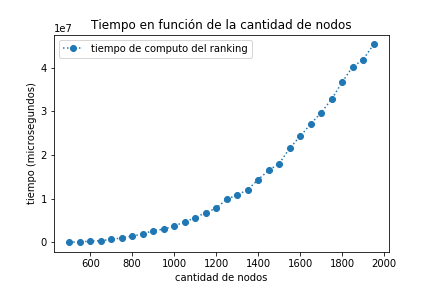
\includegraphics[width=0.475\textwidth]{img/tiempo_nodos_prop_500-2000_solo_e100.png}
                       & 
                        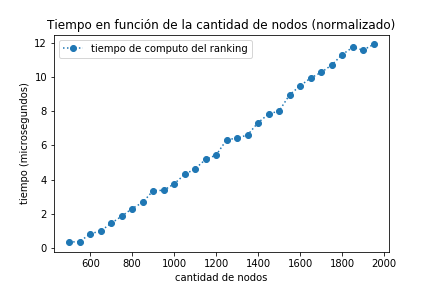
\includegraphics[width=0.475\textwidth]{img/tiempo_nodos_prop_500-2000-normalizado-e100.png}								\\
                        Con $1\%$ de ejes & Con $1\%$ de ejes normalizado por $x^{2}$ \\
                        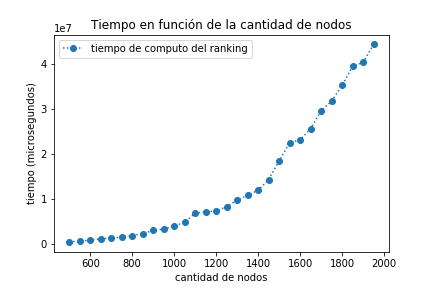
\includegraphics[width=0.475\textwidth]{img/tiempo_nodos_prop_500-2000_solo_e10.png} 
       & 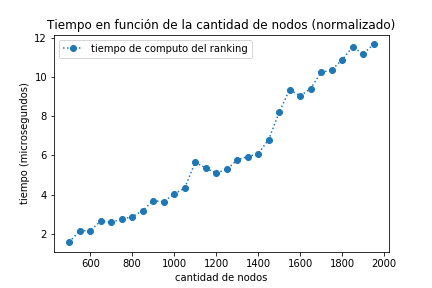
\includegraphics[width=0.475\textwidth]{img/tiempo_nodos_prop_500-2000-normalizado-e10.png} \\
             Con $10\%$ de ejes & Con $10\%$ de ejes normalizado por $x^{2}$ \\
      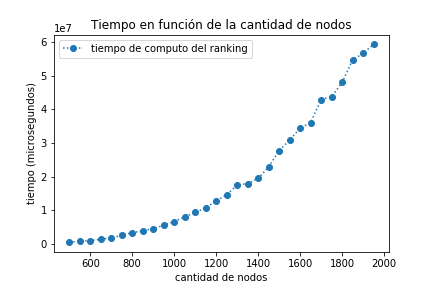
\includegraphics[width=0.475\textwidth]{img/tiempo_nodos_prop_500-2000_solo_e3.png} 
       & 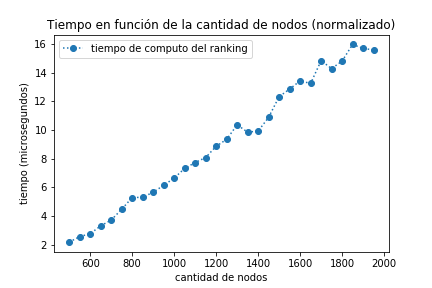
\includegraphics[width=0.475\textwidth]{img/tiempo_nodos_prop_500-2000-normalizado-e3.png} \\
             Con $33\%$ de ejes & Con $33\%$ de ejes normalizado por $x^{2}$ \\
                    \end{tabular}

                    \vspace{1em}

Resultado de la ejecución del algoritmo en función del cantidad de nodos para tres porcentajes de ejes diferentes. En las figuras de las derecha se lo normaliza por una función cuadrática.

                    \vspace{1em}
                \end{center}
                \label{fig:exp1-nodos}
            \end{minipage}

Se observa un crecimiento el tiempo de cómputo de la eliminación Gaussiana a medida que aumentamos la cantidad de páginas de la red, tal como esperábamos. La curva sugiere una función polinomial del tamaño del grafo (medido en vértices). A la derecha de cada se ilustra el mismo pero normalizado por una función cuadrática (o sea dividimos los resultados por una cuadrática sobre el rango al que aplica, en este caso 500-2000 aproximadamente). Rápidamente se visualiza una función semejante a una lineal.\\

A medida que se vuelve más densa la matriz más tarda. Esto lo vemos en más detalle con un experimento dedicado a ello a continuación. Las curvas mostradas no resultan del todo suave, en especial la del 2. Conjeturamos que se debe a la aleatoriedad de la disposición de los ejes y por lo tanto de los elementos no nulos que tiene que almacenar la matriz rala. \\

\subsubsection{Experimento 2: Variación de cantidad de Links}

Por otro lado, la iteración sobre los ejes arrojó el siguiente resultado:

\begin{figure}[H]
   \begin{center}
     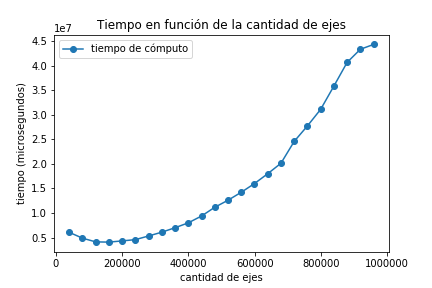
\includegraphics{img/tiempo_ejes_solo.png} 
  \end{center}
\caption{Tiempo en función de la cantidad de ejes} \label{fig:exp1-ejes}
\end{figure}

Como también se reporta en el anterior experimento, en este el costo computacional de PageRank medido en tiempo crece a medida que la red a la que se le desea calcular un ranking para determinar un orden de importancia de sus páginas se densifica. \\

Se aprecia una curva polinómica que se deriva de la mayor cantidad de elementos no nulos que la eliminación Gaussiana afronta a la hora de triangular la matriz. Existen más elementos para anular si están debajo de la diagonal, para insertar multiplicado por p y el grado del nodo de salida, cosa que conlleva una nuevas inserciones del resultado de esa cuenta en algunas filas posteriores a la suya cuando a la suya le toca ser pivot. \\
 
\newpage

\subsubsection{Experimento 3: Variación de p}


Por último, variamos p y obtuvimos lo siguiente:

\begin{figure}[H]
   \begin{center}
     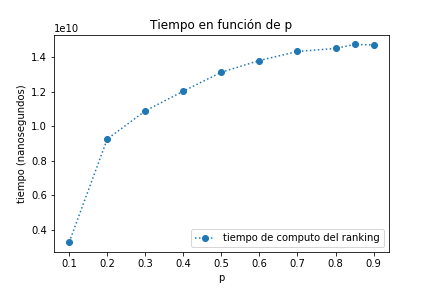
\includegraphics{img/tiempo_p.png} 
  \end{center}
\caption{Tiempo en función de p} \label{fig:exp1-p}
\end{figure}


Tal como se esperaba, a medida que crecemos el p, el requerimiento computacional del método analizado crece en una función que parece ser sublineal. Dicho crecimiento estipulamos que tiene su causa en el incremento de la cantidad de valores no nulos que han de almacenarse. Un p chico logra tender más al cero al $w_{ij}/d_{j}$ que está multiplicando y converge a su vez más rápido a lo que denominamos cero (épsilon) a medida que vamos restando valores en la ecuación de la eliminación Gaussiana $a_{ij}$ = $a_{ij}$ $-$ $\frac{a_{ik}}{a_{kk}} a_{kj}$. \\

Nótese que este resultado se encuentra relacionado con el épsilon que decidimos como cero. Otro test no reportado en el presente trabajo arrojó una función de crecimiento del tiempo de PageRank parecida a p. Es que si el épsilon es grande, muchos valores son contemplados como cero y por consiguiente la matriz almacena menos elementos no nulos y las restas de la ecuación anterior convergen más rápido y a mayor cuantía a cero. \\

\newpage

\subsection{Análisis Cualitativo}

\subsubsection{Objetivos e hipótesis:}

En la presente sección se busca analizar la calidad de los rankings calculados por el método de PageRank, evaluarlo según el contexto en el que se lo aplique y relacionándolo con la estructura del grafo subyacente a la red de páginas web a las que deseamos asignarles algún valor de preferencia. \\

Para este fin, diseñamos el siguiente conjunto de instancias.

\subsubsection{Grafo 1}


\begin{figure}[h]
     \begin{center}
     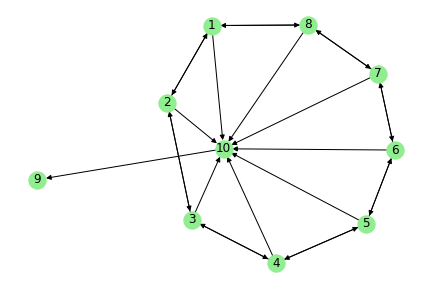
\includegraphics[scale=0.65]{img/prueba-circular.png} 
    \end{center}
\caption{Grafo 1: Un circuito fuertemente conexo conecta a un nodo y este a otro.} \label{fig:exp3-circular}
\end{figure}

Se busca con esta red evaluar el comportamiento de PageRank cuando una página con mucho grado de entrada apunta a otro que solo recibe un link de esa. De esta manera contrastamos grados vs peso del link, entre otras cosas que puedan surgir. \\

La hipótesis que planteamos es que la página nueve va ser la mas rankeada dado que la página diez es la contiene mas links y ésta sólo tiene un link hacia la página nueve, le está delegando mayor importancia y a su vez la página nueve no tiene links hacia otras páginas, por lo que no reduce su relevancia. \\

\subsubsection{Grafo 2}

\begin{figure}[H]
    \begin{center}
        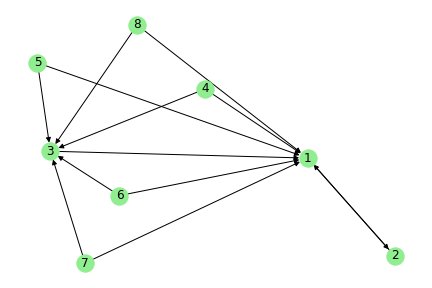
\includegraphics{img/prueba_grafo_2.png}
    \end{center}
\caption{Grafo 2: Ahora el la página que recibe un link del de mayor grado contiene un link hacia esa} \label{fig:exp3-grafo2}
\end{figure}

Aquí se busca tratar el ranking devuelto por el método para el caso donde una página muy popular en cuanto a links que la apuntan enlaza a otra y esta última le devuelve el link. Con esto creemos que se puede ver la transferencia de pesos entre los links. \\

Hipotetizamos que el puntaje otorgado a las páginas 1 y 2 son parecidos, con una leve diferencia a favor del 1 debido a la mayor cantidad de links y el hecho que otra página relevante como la 3 apunte solo a la 1. \\

\subsubsection{Grafo 3}

\begin{figure}[H]
   \begin{center}
     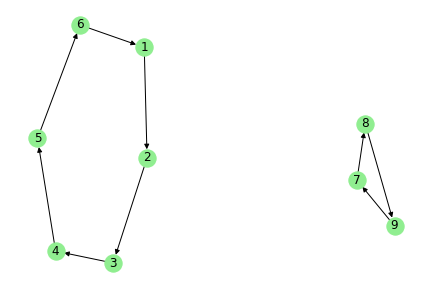
\includegraphics{img/prueba_3_no_conexa.png} 
  \end{center}
\caption{Grafo 3: Grafo de páginas no conexo.} \label{fig:exp3-noconexo}
\end{figure}

En esta experiencia se aborda el tratamiento de grafos no conexos. Cada uno es un circuito pero de distinta longitud. \\

La hipótesis plateada es que las páginas del circuito más largo lograrán un mayor puntaje. Sin embargo, también podemos pensar que dado que las páginas son referenciadas y linkeadas por una sola página, todas podrían tener la misma importancia. \\

\subsubsection{Grafo 4}

\begin{figure}[H]
   \begin{center}
     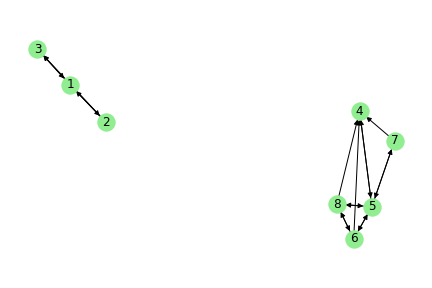
\includegraphics{img/prueba_aislado.png} 
  \end{center}
\caption{Grafo 4: 3 nodos aislados (9,10,11) no se muestran en la ilustración.} \label{fig:exp3-aislado}
\end{figure}

Este grafo amplia la desconectividad evaluada anteriormente y agrega nodos aislados. Por otra parte los dos subgrafos conexos presentan una estructura más compleja. No se aprecia tan fácilmente la página más puntuada.\\

Creemos que en una subred, 5 por ser el más apuntado, 7 por ser apuntado por este y 4 por ambos y tener pocos links de salida pelean por el primer puesto, mientras que en el otro subgrafo, el 1 parecería ser el más indicado a coronarse debido a la conexión entrante desde los otros dos vértices. En todo caso, esta es una red que creemos pareja.
Los nodos aislados deberían recibir el menor puntaje y este variar fuertemente al compás de p. \\

\subsubsection{Grafo 5}

\begin{figure}[H]
   \begin{center}
     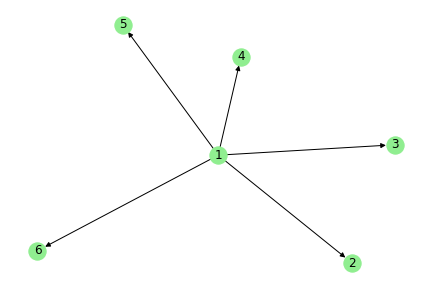
\includegraphics{img/prueba_estrella.png} 
  \end{center}
\caption{Grafo estrella: Una página apunto a todas las demás.} \label{fig:exp3-estrella}
\end{figure}

Este grafo se conoce como grafo estrella. En este caso al ser dirigido elegimos que uno apunto a todos, buscando una equivalencia de puntajes entre ellos. Al mismo tiempo también se evalua el comportamiento de una que indexa según PageRank\\

Hipotetizamos que que este las páginas que son apuntadas reciben el mismo puntaje y que la página enlazadora arroja un menor puntaje ya que nadie la linkea a pesar de ser indexadora. \\

\subsubsection{Grafo 6}

\begin{figure}[H]
   \begin{center}
     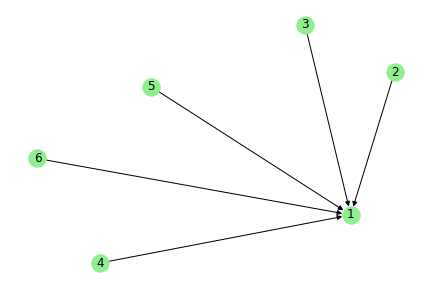
\includegraphics{img/prueba_estrella_apuntada.png} 
  \end{center}
\caption{Grafo estrella apuntada: Todas apuntan a una.} \label{fig:exp3-estrella}
\end{figure}


Aquí tenemos un grafo estrella donde todos apuntan a una misma página. \\

En el grafo estrella donde todos apuntan a una misma página, este va a ser el de mayor ranking independientemente del p que se elija. Pero este test no termina acá. Contamos con 5 grafos más. Cada uno es el resultado de agregar un eje que no estaba en el grafo y que va desde la página 1 (esa a la que enlazan todos) hasta una que no tenga grado de entrada positivo. Por lo tanto el último grafo es uno en el cual todos apuntan a uno (el 1) y este apunta a todos como se ilustra a continuación: \\

\begin{figure}[H]
   \begin{center}
     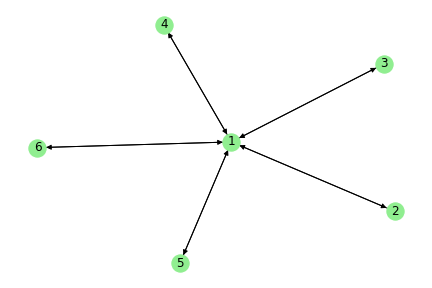
\includegraphics{img/prueba_estrella_apuntada+5.png} 
  \end{center}
\caption{Grafo estrella apuntada + 5 ejes: Todas apuntan a una y esta apunta a todas} \label{fig:exp3-estrella}
\end{figure}

En este experimento gradualista, nuestra hipótesis es que cada nuevo nodo apuntado pierde relevancia por que su enlazador debe distribuir el puntaje entre más páginas. \\\

Todos estos experimentos se corren con p = 0.3, 0.6, 0.8, 0.9 para también evaluar la influencia de la probabilidad de que el navegante aleatorio siga atrevsando la red por una página a la que la página actual enlaza.

\newpage
\subsubsection{Resultado y Análisis: }

Los resultados arrojados fueron los siguientes:

\subsubsection{Resultado Grafo 1}
\begin{center}
         \begin{tabular}{|c|c|c||c|c|c|}
                    \hline
                    \multicolumn{3}{|c||}{\emph{Ranking} Grafo 1 - \emph{p = 0.3}} & \multicolumn{3}{c|}{\emph{Ranking} Grafo 1 - \emph{p = 0.6}} \\ \hline
                    Pos. & Nodo & Puntaje    & Pos. & Nodo & Puntaje  \\ \hline
1 & 10 & 0.147059 & 1 & 10 &  0.181518 \\ 
2 & 9 & 0.117647 & 2 & 9 &  0.158416 \\
3 & 1 & 0.0919118 & 3 & 1 & 0.0825083 \\
4 & 2 & 0.0919118 & 4 & 2 & 0.0825083 \\
5 & 3 & 0.0919118 & 5 & 3 & 0.0825083 \\
6 & 4 & 0.0919118 & 6 & 4 & 0.0825083 \\
7 & 5 & 0.0919118 & 7 & 5 & 0.0825083 \\
8 & 6 & 0.0919118 & 8 & 6 & 0.0825083 \\
9 & 7 & 0.0919118 & 9 & 7 & 0.0825083 \\
10 & 8 & 0.0919118 & 10 & 8  & 0.0825083 \\ \hline
                    \multicolumn{6}{c}{} \\ \hline
                    \multicolumn{3}{|c||}{\emph{Ranking} Grafo 1 - \emph{p = 0.8}} & \multicolumn{3}{c|}{\emph{Ranking} Grafo 1 - \emph{p = 0.9}} \\ \hline
                    Pos. & Nodo & Puntaje    & Pos. & Nodo & Puntaje  \\ \hline
1 & 10 & 0.197769  & 1 & 9 &  0.212828 \\ 
2 & 9 & 0.193712  & 2 & 10 &  0.204082 \\
3 & 1 & 0.0760649  & 3 & 1 & 0.0728863 \\
4 & 2 & 0.0760649  & 4 & 2 & 0.0728863 \\
5 & 3 & 0.0760649  & 5 & 3 & 0.0728863 \\
6 & 4 & 0.0760649  & 6 & 4 & 0.0728863 \\
7 & 5 & 0.0760649  & 7 & 5 & 0.0728863 \\
8 & 6 & 0.0760649  & 8 & 6 & 0.0728863 \\
9 & 7 & 0.0760649  & 9 & 7 & 0.0728863 \\
10 & 8 & 0.0760649 & 10 & 8  & 0.0728863 \\ \hline

                \end{tabular}
            \end{center}

Vemos que en los primeros 3 \textit{p} la página lider es la 10, que es la de mayor grado de entrada. Con p = 0.9 la página 9 que solo es apuntada por la 10 pasa al frente con cierta diferencia. Esto se debe a que con mayor probabilidad de pasar de una página a otro a través de uno de sus enlaces más en cuenta se tiene la estructura de la red. Como la página 10 es la a la que más se apunta (todos lo hacen menos la 9), esta es una página importante y al encontrarse enlazando a la 9 le transfiere un gran peso a través de dicho link. \\

A su vez todo el puntaje del nodo 10 se pondera en el mencionado enlace ya que no apunta a otra página. Solo a la 9. \\
En cuanto al resto de los nodos, poseen siempre el mismo puntaje porque solo reciben un link y de páginas como ellos. Ninguno de 10 ni de 9. Por lo tanto el peso de esos links es el mismo y es bastante pobre comparado con el eje previamente mencionado. \\

Por último, se puede observar que a medida que aumentamos el p baja el puntaje de las paginas 1-8. La razón es la misma que la expuesta previamente. Al ponderar más la topología del grafo, mayor valor tienen los enlaces fuertes como el del 10 al 9 y el grado de entrada de 10. Esto sucede en detrimento del ranking de los nodos 1-8. Al estar un navegante aleatorio 9 de cada 10 veces en caso de p = 0.9 eligiendo las páginas a las que enlaza la actual en donde esta parado, entonces mayor es la probabilidad de que este atraviese uno de los links que lo lleve a una página popular dentro de la red (como es el caso de la 10 donde 7 páginas lo apuntan) y además, mayor es la probabilidad de parar en la página 9 ya que la probabilidad de estar en la 10 es alta y esta solo tiene un enlace a 9. Como 9 de cada 10 veces se elige seguir el recorrido virtual atrevesando un link, entonces es bastante probable que se visite la página 9. \\

Esto se puede deducir a su vez de las ecuaciones del PageRank. Si se esta en una página entre la 1-8, es equiprobable que se siga la navegación en la página web 10 o en otra a la que la página en cuestión apunte. Por lo que solo se divide por dos en la sumatoria de los pesos de las aristas que apuntan al nodo 10 y nadie entre el 1-8 y 10 ostenta mayor grado de entrada que la 10. \\

Por otra parte, como solo 10 apunta a 9, al peso de 10 solo se lo divide por 1. Se transfiere así el puntaje de 10 en su totalidad ponderado en exclusivo por el p escogido. Si se quiere menor desigualdad de puntaje se decrementa el p como vimos antes. Asimismo se puede reducir el valor de p con el fin de que el navegante quede estancado un tiempo largo en la página 9, que es la única que no posee enlaces de salida. \\

Nos podemos preguntar que interpretación a través el cristal de un motor de búsqueda temática emerge de lo discutido. En este grafo, PageRank empareja una página que recibe muchos links con una que solo recibe un link proveniente de la más popular. \\ 
Por un lado la web más popular de un conjunto puede no tener relación con lo buscado. Solo nos deriva a la de mayor peso y quizás una apuntada específicamente por esta podría ser más autoritativa en el tópico deseado. La página derivada de la más popular (en este caso 9 que deriva de 10) podría ser de carácter más preciso en relación a lo solicitado.\\

Por otro lado si la red se arma a partir de un filtrado de paginas relacionadas entre sí (como por ejemplo un filtrado temático basado en la correspondencia de palabras buscadas con el nombre de la página y el parseo de algunos contenidos de la misma, entre otras métricas posibles) tal vez la página más enlazada y, que además es linkeada por páginas con puntaje importante en relación a esta red, sea la que más se aproxima a lo pretendido por quien busca un tema específico.\\

La página 9 apuntada en solitario por la 10 podría no ser relevante en el tópico y solo estar inflada debido a que su enlazador es la más popular. Este creemos que es un problema en algunos contextos donde PageRank calcula el ranking. Por ejemplo, se puede considerar a 10 como un sitio importante en la materia y 9 como uno sitio al que solo enlaza a través de una publicidad que 9 le paga a 10 para otorgarse importancia. 9 sabe que 10 es popular dentro de una comunidad y desea aprovechar esto para su beneficio. Esa ambigüedad puede ser un punto en contra del método.\\

Creemos entonces que contexto de aplicación de PageRank para un caso como el grafo descripto condiciona la calidad del ranking obtenido. \\

\subsubsection{Resultado Grafo 2}

\begin{center}
         \begin{tabular}{|c|c|c||c|c|c|}
                    \hline
                    \multicolumn{3}{|c||}{\emph{Ranking} Grafo 2 - \emph{p = 0.3}} & \multicolumn{3}{c|}{\emph{Ranking} Grafo 2 - \emph{p = 0.6}} \\ \hline
                    Pos. & Nodo & Puntaje    & Pos. & Nodo & Puntaje  \\ \hline
1 & 1 &  0.247596 & 1 & 1 & 0.359375 \\ 
2 & 2 &  0.161779 & 2 & 2 & 0.265625 \\
3 & 3 &  0.153125  & 3 & 3 & 0.125 \\
4 & 4 &  0.0875  & 4 & 4 &  0.05 \\
5 & 5 &  0.0875  & 5 & 5 &  0.05 \\
6 & 6 &  0.0875  & 6 & 6 &  0.05 \\
7 & 7 &  0.0875  & 7 & 7 &  0.05 \\
8 & 8 &  0.0875  & 8 & 8 &  0.05 \\
 \\ \hline
                    \multicolumn{6}{c}{} \\ \hline
                    \multicolumn{3}{|c||}{\emph{Ranking} Grafo 2 - \emph{p = 0.8}} & \multicolumn{3}{c|}{\emph{Ranking} Grafo 2 - \emph{p = 0.9}} \\ \hline
                    Pos. & Nodo & Puntaje    & Pos. & Nodo & Puntaje  \\ \hline
1 & 1 & 0.430556 & 1 & 1 & 0.465461 \\ 
2 & 2 & 0.369444 & 2 & 2 & 0.431414 \\
3 & 3 & 0.075  & 3 & 3 & 0.040625 \\
4 & 4 & 0.025  & 4 & 4 & 0.0125 \\
5 & 5 & 0.025  & 5 & 5 & 0.0125 \\
6 & 6 & 0.025  & 6 & 6 & 0.0125 \\
7 & 7 & 0.025  & 7 & 7 & 0.0125 \\
8 & 8 & 0.025  & 8 & 8 & 0.0125 \\

 \\ \hline

                \end{tabular}
            \end{center}
   
En este grafo a medida que aumentamos p, más se decrece la diferencia del nodo 2 con el 1, que es el de mayor grado de entrada. Es notable tambíen como el nodo 3 con p = 0.3 ostenta un puntaje no tan distinto del 2 pero esta diferencia crece ostensiblemente a medida que ponderamos más el entramado del grafo aumentando p. \\

Otra vez los nodos más desfavorecidos (4-8), que reciben el mismo puntaje entre ellos en cada corrida, disminuyen su score a medida que aumentamos p. Creíamos que 3 podía escapar de esta lógica al ser una página apuntada por casi todos. Sin embargo, analizando detenidamente el grafo y relacionándolo con las ecuaciones del PageRank, los mismos que apuntan a 1 apuntan a 3, pero este último apunta al primero y el primero no lo apunta a él si no al 2. \\

Por lo tanto el 3 transfiere autoridad acumulada a través de su único enlace en la red. Y el destino de este link es 1. Este entonces recibe los mismos enlace que 3 y a todo el peso de 3. El 2 por su parte recibe un link del 1 pero este a su vez se lo refleja. Ninguno de los dos posee otros links de salida por lo que se puede describir este ciclo como una retroalimentación. Solo por que posee otros enlaces entrantes es el 1 algo mejor puntuado que la página 2. \\

Si de sitios webs se trata, nos resulta exagerada la poca relevancia que PageRank le otorga al 3. Su puntaje es hasta 10 veces menor que el 2 si se considera un alto p.\\
A diferencia del anterior grafo y a favor de PageRank podemos decir que si 2 ahora enlaza a 1 entonces el vínculo entre estas páginas es más fuerte. Difícilmente un caso como el descripto anteriormente pueda darse. El nexo temático nos parece más factible en esta estructura de red y PageRank logra capturarlo. \\

\subsubsection{Resultado Grafo 3}   
            

\begin{center}
         \begin{tabular}{|c|c|c|}
                    \hline
                    \multicolumn{3}{|c||}{\emph{Ranking} Grafo 3 - \emph{p = 0.3, 0.6, 0.8, 0.9}} \\ \hline
Pos. & Nodo & Puntaje \\ \hline
1 & 1 & 0.111111 \\ 
2 & 2 & 0.111111 \\
3 & 3 & 0.111111 \\
4 & 4 & 0.111111 \\
5 & 5 & 0.111111  \\
6 & 6 & 0.111111  \\
7 & 7 & 0.111111   \\
8 & 8 & 0.111111 \\
9 & 9 & 0.111111  \\
 \hline

                \end{tabular}
            \end{center}
 
Para nuestra sorpresa el puntaje otorgado por PageRank a los distintos nodos es el mismo. Con lo cual es equiprobable partiendo de cualquier página terminar en cualquier otra. Analizando cuidadosamente la ecuación que define el score vemos que solo depende del peso del link de entrada. Cada vértice tiene un eje entrante y uno saliente por lo que la única ponderación es el p. El score se propaga a través del subgrafo que es un circuito dirigido por lo que todos reciben el mismo. En ningún lado se hace mención a la cantidad de páginas involucradas en este. \\

Como se observa, PageRank no distingue entre el tamaño de cada circuito. Todos tienen el mismo grado de entrada y de salida. Dada esta curiosidad experimentamos con el mismo grafo pero completo en cada componente conexa. El resultado fue el mismo. Y probamos también en un caso de mayor diferencia. Un digrafo $K_{2}$ completo y otro $K_{7}$. Arrojó el exactamente el mismo resultado. \\

Este comportamiento de PageRank de alguna manera ilustra lo que denominamos transferencia de peso, poder o importancia entre los nodos. Toda página vale del score de todas las demás en esa componente conexa por lo que se divide el puntaje entre todas. \\

Una consideración que nos surge es cómo determinamos la importancia relativa entre dos componentes conexas. Si en un conjunto de páginas no hay links entre dos subconjuntos, ¿cómo determinamos cuál es más relevante?. Múltiples propuestas se desprenden de esta pregunta. Puede ponderarse la de mayor cantidad de páginas o links entre ellas. O como realiza PageRank, que pondera los enlaces en relación al puntaje de la página enlazadora. Pero si tenemos un caso como este,
entonces no escapa de la equiprobabilidad.\\

Creemos que una comunidad de sitios web representada como subgrafo conexo de mayor cantidad de páginas debería tener más relevancia que una comunidad más chica. Esto PageRank no lo captura y otorga el mismo puntaje a todas las páginas en una búsqueda temática. \\
            
\subsubsection{Resultado Grafo 4} 

\begin{center}
         \begin{tabular}{|c|c|c||c|c|c|}
                    \hline
                    \multicolumn{3}{|c||}{\emph{Ranking} Grafo 4 - \emph{p = 0.3}} & \multicolumn{3}{c|}{\emph{Ranking} Grafo 4 - \emph{p = 0.6}} \\ \hline
                    Pos. & Nodo & Puntaje    & Pos. & Nodo & Puntaje  \\ \hline
1 & 5 & 0.131359 & 1 & 5 & 0.174397 \\ 
2 & 1 & 0.111924 & 2 & 1 & 0.133779 \\
3 & 4 & 0.108624  & 3 & 4 & 0.125348 \\
4 & 3 & 0.0990099  & 4 & 3 & 0.108696 \\
5 &  6 & 0.0879543 & 5 & 6 & 0.0870474 \\
6 & 8 & 0.0879543  & 6 & 8 & 0.0870474 \\
7 & 2 & 0.0860956  & 7 & 2 & 0.083612 \\
8 &  7 & 0.0791588 & 8 & 7 & 0.0696379 \\
9 &  9 & 0.0693069 & 9 & 9 & 0.0434783 \\
10 & 10 & 0.0693069  & 10 & 10 & 0.0434783\\
11 & 11 & 0.0693069  & 11 & 11 & 0.0434783 \\ \hline
                    \multicolumn{6}{c}{} \\ \hline
                    \multicolumn{3}{|c||}{\emph{Ranking} Grafo 4 - \emph{p = 0.8}} & \multicolumn{3}{c|}{\emph{Ranking} Grafo 4 - \emph{p = 0.9}} \\ \hline
                    Pos. & Nodo & Puntaje    & Pos. & Nodo & Puntaje  \\ \hline
1 & 5 & 0.205095 & 1 & 5 & 0.221261 \\ 
2 & 1 & 0.149502 & 2 & 1 & 0.157873 \\
3 & 4 & 0.13673  & 3 & 4 & 0.142655 \\
4 & 3 & 0.116279  & 4 & 3 & 0.120482 \\
5 &  6 & 0.0876475 & 5 & 6 & 0.0883312 \\
6 & 8 & 0.0876475 & 6 & 8 & 0.0883312 \\
7 & 2 & 0.0830565  & 7 & 2 & 0.083091 \\
8 &  7 & 0.0642749 & 8 & 7 & 0.0618318 \\
9 &  9 & 0.0232558& 9 & 9 & 0.0120482 \\
10 & 10 & 0.0232558  & 10 & 10 & 0.0120482\\
11 & 11 & 0.0232558  & 11 & 11 & 0.0120482 \\ \hline

                \end{tabular}
            \end{center}
            
Este grafo contiene 3 nodos aislados, 9, 10 y 11. Como en el anterior grafo, existen dos componentes conexas. Sin embargo la estructura de ambos subgrafos conexos es distinta. En la subred más poblada 5 resulta ser el más valorado por PageRank. Es a su vez al que todas las páginas de la red apuntan. Si bien el vértice 4 recibe un enlace de todos los nodos de ese subgrafo, este no hace lo mismo y mantiene un solo enlace de salida que apunta a 5. \\

De esta manera, 4 es solo realimentado por 5, mientras que este último es realimentado por todo el subgrafo. Esta noción puede explicarse por las ecuaciones. Como el puntaje de la página 5 depende de todos los que lo apuntan y a su vez el puntaje de esos depende del puntaje de el nodo 5 (ya que este posee links hacia ellos) entonces entendemos que PageRank logra que la página 5 se reatroalimente de su propio puntaje. \\

A nuestro criterio esto logra que un sitio web autoritativo en la materia obtenga una posición merecedora en el ranking armado por el algoritmo de PageRank. Es que una web así puede pensarse sumamente influyente dentro de una comunidad vinculada al tópico que se desa encontrar. Sirve como puente e introducción a las demás y estas a su vez la conocen, la linkean. Se puede interpretar una página como la 5 como poderosa en el marco de cierto dominio, tanto para delegar conocimiento como referencia en un área. \\

Una objeción que puede surgir es una página de dichas características ha de ser leida como una importante pero generalista. Pueden ser buscadores / indexadores y todos la apuntan por ese motivo: sirve para que las hagan conocidas. A su vez esta página que puede ser un portal o sitio de noticias enlaza a las otras con el fin de capturar alguna porción del tráfico que busca asunto determinado. Claramente este "pulpo" no sería la mejor opción en un ranking ponderado por la materia que se desea encontrar en la web .\\

Por otra lado, el nodo 1 se gana el segundo lugar en el ranking para cualquier p. A pesar de contar con solo dos links de entrada, el feedback es fuerte ya que esas dos páginas son enlazadas por esta misma. A medida que se tiene más en cuenta la estructura del grafo, aumentando p, disminuye su relación de fuerza respecto al nodo 5 pero le saca mayor ventaja al resto.
Esta sobrevaloración de una página que se retroalimenta de pocas y que pertenece a una componente conexa mucho más pequeña que otra, como es el caso del subrafo al que pertenece el sitio 5 donde varios nodos tienen más enlaces, se antoja como una debilidad del ranking de PageRank y de esa manera lo notamos nosotros. \\

Por último y como era de esperarse, los vértices aislados son asignados a los puestos más bajos del ranking. Se cumple la lógica en este caso y es deseable que así sea ya que páginas a las que ninguna cita y ni siquiera estas se conectan con algún otra de la red, no parecen ser una envidiable muestra de envergadura en la materia buscada.\\ 
  
            
\subsubsection{Resultado Grafo 5: Estrella saliente} 

\begin{center}
         \begin{tabular}{|c|c|c||c|c|c|}
                    \hline
                    \multicolumn{3}{|c||}{\emph{Ranking} Grafo Estrella - \emph{p = 0.3}} & \multicolumn{3}{c|}{\emph{Ranking} Grafo Estrella - \emph{p = 0.6}} \\ \hline
                    Pos. & Nodo & Puntaje    & Pos. & Nodo & Puntaje  \\ \hline
1 & 2 & 0.168254 & 1 & 2 & 0.169697 \\ 
2 & 3 & 0.168254 & 2 & 3 & 0.169697 \\
3 & 4 & 0.168254  & 3 & 4 & 0.169697 \\
4 & 5 & 0.168254  & 4 & 5 & 0.169697 \\
5 &  6 & 0.168254 & 5 & 6 &  0.169697 \\
6 & 1 & 0 0.15873 & 6 & 1 &  0.151515 \\ \hline
                    \multicolumn{6}{c}{} \\ \hline
                    \multicolumn{3}{|c||}{\emph{Ranking} Grafo Estrella - \emph{p = 0.8}} & \multicolumn{3}{c|}{\emph{Ranking} Grafo Estrella - \emph{p = 0.9}} \\ \hline
                    Pos. & Nodo & Puntaje    & Pos. & Nodo & Puntaje  \\ \hline
1 & 2 & 0.170588 & 1 & 2 & 0.171014 \\ 
2 & 3 & 0.170588 & 2 & 3 & 0.171014 \\
3 & 4 & 0.170588  & 3 & 4 & 0.171014 \\
4 & 5 & 0.170588  & 4 & 5 & 0.171014 \\
5 &  6 & 0.170588 & 5 & 6 &  0.171014 \\
6 & 1 & 00.147059 & 6 & 1 &  0.144928 \\ \hline

                \end{tabular}
            \end{center}
            
Este grafo puede leerse como una representación de un indexador. Puede considerarse una página de esta índole como destacada por el simple hecho de ser un canal de retransmisión de información. Pero como sitio autoritativo en la materia no tanto. Creemos que son más importantes las apuntadas por este. \\

El ranking concebido por PageRank no otorga demasiadas pistas sobre qué paginas pueden resultar útiles pero destacamos que al menos no sobrevalora a un indexador que podría ser considerado poderoso en otras circunstancias y en diferentes métodos de oredanamiento de páginas webs. \\
Notar que incluso aunque sea un buscador o redireccionador exclusivamente de contenidos que abarquen a lo pretendido, los sitios enlazados por este serán lógicamente de mayor relevancia y esto es capturado por PageRank.\\

\textit{p} por su parte juega el mismo papel que en los experimentos predecesores. A medida que aumenta más énfasis se hace sobre la estructura del grafo, en particular, su conectividad. \\
            
\subsubsection{Resultado Grafo 6: Etrella entrante} 

\begin{center}
         \begin{tabular}{|c|c|c||c|c|c|}
                    \hline
                    \multicolumn{3}{|c||}{\emph{Ranking} Grafo Estrella Entrante - \emph{p = 0.3}} & \multicolumn{3}{c|}{\emph{Ranking} Grafo Estrella entrante - \emph{p = 0.9}} \\ \hline
                    Pos. & Nodo & Puntaje    & Pos. & Nodo & Puntaje  \\ \hline
1 & 1 & 0.333333 & 1 & 1 & 0.52381 \\ 
2 & 2 & 0.133333 & 2 & 2 & 0.0952381 \\
3 & 3 & 0.133333  & 3 & 3 & 0.0952381 \\
4 & 4 & 0.133333  & 4 & 4 & 0.0952381 \\
5 &  5 & 0.133333 & 5 & 5 &  0.0952381\\
6 & 6 & 0.133333 & 6 & 6 & 0.0952381 \\
 \hline
                    \multicolumn{3}{c}{} \\ \hline
                    \multicolumn{3}{|c||}{\emph{Ranking} Grafo estrella 1 eje - \emph{p = 0.3}} & \multicolumn{3}{c|}{\emph{Ranking} Grafo estrella entrante 1 eje - \emph{p = 0.9}} \\ \hline
                    Pos. & Nodo & Puntaje    & Pos. & Nodo & Puntaje  \\ \hline
1 & 1 & 0.320513 & 1 & 1 & 0.482456 \\ 
2 & 6 & 0.212821 & 2 & 6 &  0.450877 \\
3 & 2 & 0.116667  & 3 & 2 & 0.0166667 \\
4 & 3 & 0.116667  & 4 & 3 & 0.0166667 \\
5 &  4 & 0.116667 & 5 & 4 &  0.0166667 \\
6 & 5 & 0.116667 & 6 & 5 & 0.0166667 \\
 \hline
 
                    \multicolumn{3}{c}{} \\ \hline
                    \multicolumn{3}{|c||}{\emph{Ranking} Grafo estrella 2 ejes - \emph{p = 0.3}} & \multicolumn{3}{c|}{\emph{Ranking} Grafo estrella entrante 2 ejes - \emph{p = 0.9}} \\ \hline
                    Pos. & Nodo & Puntaje    & Pos. & Nodo & Puntaje  \\ \hline 
 1 & 1 & 0.320513 & 1 & 1 & 0.482456 \\ 
2 & 5 & 0.164744 & 2 & 6 &  0.233772 \\
3 & 6 & 0.164744  & 3 & 2 &  0.233772 \\
4 & 2 & 0.116667  & 4 & 3 & 0.0166667 \\
5 &  3 & 0.116667 & 5 & 4 &  0.0166667 \\
6 & 4 & 0.116667 & 6 & 5 & 0.0166667 \\ \hline

                    \multicolumn{3}{c}{} \\ \hline
                    \multicolumn{3}{|c||}{\emph{Ranking} Grafo estrella 3 ejes - \emph{p = 0.3}} & \multicolumn{3}{c|}{\emph{Ranking} Grafo estrella entrante 3 ejes - \emph{p = 0.9}} \\ \hline
                    Pos. & Nodo & Puntaje    & Pos. & Nodo & Puntaje  \\ \hline 


1 & 1 & 0.320513 & 1 & 1 & 0.482456 \\ 
2 & 4 & 0.148718 & 2 & 4 &  0.161404 \\
3 & 5 & 0.148718  & 3 & 5 &  0.161404 \\
4 & 6 & 0.148718  & 4 & 6 &  0.161404 \\
5 & 2 & 0.116667 & 5 & 2 &  0.0166667 \\
6 & 3 & 0.116667 & 6 & 3 & 0.0166667 \\ \hline

                    \multicolumn{3}{c}{} \\ \hline
                    \multicolumn{3}{|c||}{\emph{Ranking} Grafo estrella 4 ejes - \emph{p = 0.3}} & \multicolumn{3}{c|}{\emph{Ranking} Grafo estrella entrante 4 ejes - \emph{p = 0.9}} \\ \hline
                    Pos. & Nodo & Puntaje    & Pos. & Nodo & Puntaje  \\ \hline 

1 & 1 & 0.320513 & 1 & 1 & 0.482456 \\ 
2 & 3 & 0.140705 & 2 & 3 &  0.125219 \\
3 & 4 & 0.140705  & 3 & 4 &  0.125219 \\
4 & 5 & 0.140705  & 4 & 5 &  0.125219 \\
5 & 6 & 0.140705 & 5 & 6 &  00.125219 \\
6 & 2 & 0.116667 & 6 & 2 & 0.0166667 \\ \hline

                    \multicolumn{3}{c}{} \\ \hline
                    \multicolumn{3}{|c||}{\emph{Ranking} Grafo estrella 5 ejes - \emph{p = 0.3}} & \multicolumn{3}{c|}{\emph{Ranking} Grafo estrella entrante 5 ejes - \emph{p = 0.9}} \\ \hline
                    Pos. & Nodo & Puntaje    & Pos. & Nodo & Puntaje  \\ \hline 

1 & 1 & 0.320513 & 1 & 1 & 0.482456 \\ 
2 & 2 & 0.135897 & 2 & 2 &  0.103509 \\
3 & 3 & 0.135897  & 3 & 3 &  0.103509 \\
4 & 4 & 0.135897  & 4 & 4 &  0.103509 \\
5 & 5 & 0.135897 & 5 & 5 &  00.103509 \\
6 & 6 & 0.135897 & 6 & 6 & 00.103509 \\ \hline

                \end{tabular}
            \end{center} 
            
Para terminar, analizamos los resultados arrojados por correr PageRank sobre un grafo estrella al que uno es apuntado por todos. Lo buscado en verdad no es esto sino la tranformación del ranking a medida que se agrega un eje del más apuntado a uno que no es enlazado por ningun otro. Para simplificar su visualización solo se muestran los casos para p = 0.3 y p = 0.9. 
p cumple el mismo rol que reiteramos con anterioridad en otras experiencias y creemos que con tomar los dos extremos alcanza para analizar esta prueba. \\

En el primer caso, cuando todos apuntan a la página 1, esta recibe el mayor puntaje como es de esperarse. Con p = 0.9 la probabilidad parar en la página 1 es mayor a 0.5. \\
Cuando agregamos un eje entre 1 y 6, esta última trepa a casi el puntaje de 1 para p = 0.9. Es decir, si se pondera mucho la estructurade la red, la página 6 a la que solo apunta la página 1 escala hasta casi alcanzarla. Esto se puede explicar por la ya expuesto antes. El link de entrante a 6 otorga todo el puntaje de 1, pesado por p. Pero como el sitio 6 enlaza al 1, este último se retroalimenta ya que ahora 6 cuenta con el puntaje de 1 ponderado. Como además a 1 lo apunta también el resto de la red, este se mantiene primero en el ranking, aunque con menor puntaje debido al grado de salida positivo que ahora posee y la consecuente transferencia de score. \\

Se podría argumentar que en esta red el más influyente sigue siendo el nodo 1. Todos lo conectan. Pagerank tiene la tendencia de otorgarle un gran puntaje a aquellas páginas que son apuntadas por nodos importantes. En este caso un link proveniente del sitio mejor puntuado de este conjunto alcanzan para casi equiprar a la página 6 con la 1, la página de mayor importancia. \\

Desde un punto de vista, el sitio 1 ni siquiera tendría por qué ser el que mejor se corresponde con un dominio específico. Si este es solo una página popular y es por eso que la linkean varias otras independientemente del tema que se maneje, entonces este problema constituye uno estructural a la concepción de PageRank. No vislumbramos una salida sencilla al mismo y como muchas decisiones que se toman, acrrean sus puntos a favor y en contra. Pero creemos que valiéndose de un preprocesamiento adecuado de los sitios que los agrupes por ejemplo según una correspondencia linguística, entnces PageRank logra un ranking bastante justo para este caso en el que todos apuntan a una. Nos da una buena pista de por cuál sitio empezar. \\

Lo realmente interesante viene en los experimentos siguientes. 1 ahora enlaza a a 5. Este sube su puntaje y escala puestos pero no obtiene el mismo puntaje que 6 en el grafo anterior sino casi la mitad.\\
Este fenómeno se debe a que ahora el puntaje de la página 1 se lo dividen entre la página 6 y la página 5. Por consiguiente, cada una recibe el mismo puntaje. Como ambas apuntan a 1, esta última no ve modificado su puntaje. El puntaje que vuelve al nodo 1 en el grafo anterior de la mano del sitio 6, es devuelto ahora por la suma de los enlaces (5,1) y (6,1). \\

A medida que se agrega un link desde la página 1 hasta otra página j que no lo tiene, aumenta el puntaje de j en detrimento de los demás menos del 1. (tanto de los que ya tienen un enlace proveniente del nodo 1 , que ven disminuido su ranking por el reparte del puntaje de este último al estar ponderado este por el grado saliente, como de los que todavía no poseen un link entrante proveniente del sitio 1 - debido a la menor importancia relativa que ostentan estos ahora en compración con los que ya tienen un link ). El score del vértice 1 no se ve modificado por lo explicado arriba.  \\

En el último caso, todos poseen el mismo puntaje salvo la página 1, ya que es la de mayor grado de entrada. \\
Por lo tanto, en este test se visualizó la noción de que conviene que apunten nodos importantes y que estos no tengan un grado de salida muy grande para así recibir buena parte del puntaje de tal nodo relevante. \\           
                                               
\newpage

\section{Conclusión}

En el presente trabajo analizamos el método de PageRank con el fin de ordenar un conjunto de páginas webs. Para ello intrujimos el modelo de navegante aleatorio que, basándose en estudios del comportamiento de un usuario al recorrer la web, mejora el PageRank al asignarle una probabilidad p a la siguiente página que el navegante decide visitar a través de uno de los enlaces de la página en la que esta parado.\\
De esta manera se logra evitar quedarse estancado en un sitio que no posee links salientes y además le otorga granularidad al peso que posee la estructura del grafo que describe la red.\\
Para calcular este ranking que pondera el puntaje de la página enlazadora y su grado de salida en cada link entrante, se debe resolver un sistema de ecuaciones lineales. Teniendo en cuenta los pocos links que suelen existir en una red en relación a su tamaño, implementamos el algoritmo de Eliminación Gaussiana sobre una matriz rala con el fin de garantizar una mayor eficiencia del método.\\

Se contrastó empíricamente la eficiencia de tal representación variando la cantidad de nodos y ejes del grafo de la red de páginas, dando como resultado un menor requerimiento de computacional a nivel temporal en función del tamaño de la matriz cuando, enespecial cuando la cantidad de ejes es poca en relación a la cantidad de nodos. \\
A su vez se evaluó cómo afecta la probabilidad p al tiempo demandado por el método, dando como resultado un incremento del mismo a medida que dicha probabilidad aumentaba. Esto a la mayor cantidad de elementos no nulos que la matriz rala debe almacenar al estar sus valore más alejados del cero definido por nosotros. \\

Luego se probó PageRank en una serie de redes elegidas cuidadosamente para resaltar la esencia de este ranking. \\
Vimos que efectivamente este no solo toma en cuenta el grado de entrada de un nodo sino el puntaje que le aportan cada una de esas páginas que lo apuntan. Ese es el caso de la primera red testeada, en la cual una página que solo recibía un enlace de la páginas mejor úbicada (que a su vez era la más popular en cuenta a grado de entrada se refiere) le disputaba el primer puesto a esta última.\\
A raiz de esto discutimos acerca de la contextualización del uso de PageRank y su valorización. Esta esencia del PageRank que pondera los enlaces por el puntaje de las páginas enlazadoras puede filtrar muchas páginas irrelevantes en la tématica buscada y subir el puntaje no solo a las que reciben muchos links sino a las que reciben de otros sitios importantes de la red. Si bien creemos que esto es más justo que medir solo el grado de entrada, se debe tener cuidado en ciertos contextos como aquel en el cual una página linkea a otra por publicidad sin tener relación alguna con el tópico de la página, ni el buscado por usuario. \\

Luego se observó cierta trasnferencia de puntaje y retroalimentación en la valoración de una página que recibe links de sitios a los que esta apunta. A veces esto puede llevar a una sobrevaloración de los nodos involucrados en detrimento de otros sin este feedback pero con varios enlaces de relativa importancia. Si bien esto puede dejar relagada algunas páginas temáticas, creemos que la existencia de un doble enlace entre páginas importantes sugieren una conexión en cuento al contenido de las mismas y esto puede verse reflejado aprovechando el rasgo retroalimentación de PageRank. \\

En redes no conexas con igua cantidad de enlaces entre sí en cada componente, PageRank optó por equiprobabilidad a lo largo de toda la red. En nuestra opinión esto constituye una debilidad del método ya que subgrafos conexos más grandes infieren cierta relación entre los mismos que puede usarse para ordenar un resultado de búsqueda. \\

Los nodos aislados son relegados adecuadamente por PageRank. En otro test, esa retroalimentación descripta arriba resultó ser algo excesiva a nuestros ojos ya que una página con pocos links de entrada casi empardaba el puntaje de otra de mayor grado de entrada. Aún así, \\

Por otro lado, vimos que PageRank captura correctamente la noción de indexador y no le otorga tanta relevancia como aquellas páginas webs que indexa. \\
Por su parte, el aumento de la probabilidad p de transición a una página enlazada por la actual siempre redundó en una mayor desigualdad entre las mejores páginas ubicadas en el ranking y las peores ya que a mayor p más se tiene en cuenta la estructura de la red. Al ser p pequeño existen más saltos aleatorios entre páginas no necesariamente enlazadas, aumentando así el puntaje de las páginas más desfavorecidas.

Por último, se comprobó la importancia que le asigna al grado de salida del nodo enlazador. La distribución del puntaje del mismo en varios nodos reduce el puntaje de quienes lo recepcionan. Puede verse esto también como una disminución de la relevancia transferida por una página a otra. Esta propiedad es la esencia de PageRank. \\


Concluimos entonces que el método de tales características resumidas aquí y desarrolladas en el pesente trabajo a partir de los experimentos previamente documentados ha de utilizarse con criterio, contextualizando su uso y combinándolo con otras métricas que se adapten a un dominio específico con el fin de elebarorar un ranking de páginas webs importantes para ser devueltos por un motor de búsqueda.\\

Queda pendiente para trabajos posteriores la corrida de PageRank sobre bases temáticas reales de miles de páginas con el fin de determinar su comportamiento en un escenario más aproximado al mundo real. \\

Otros posibles trabajos pueden abordar otras aplicaicones de PageRank, la confecicón de un ranking deportivo. \\
\newpage

\section{Referencias}

 
\begin{thebibliography}{9}


\bibitem{burden} 
R. Burden y J.D.Faires,  \textit{Análisis numérico}, International Thomson Editors, 1998

\end{thebibliography}

\newpage

\section{Apéndice} \label{cap:apendice}


%\newpage

\end{document}
